% ============================================================================
% IEEE Conference Paper: NeuroStep - Autism Detection Using ML
% Compile with: pdflatex ieee_paper.tex && bibtex ieee_paper && pdflatex ieee_paper.tex && pdflatex ieee_paper.tex
% ============================================================================
\documentclass[conference]{IEEEtran}

% --- Essential Packages ---
\usepackage{cite}
\usepackage{amsmath,amssymb,amsfonts}
\usepackage{algorithmic}
\usepackage{algorithm}
\usepackage{graphicx}
\usepackage{textcomp}
\usepackage{xcolor}
\usepackage{booktabs}
\usepackage{multirow}
\usepackage{hyperref}
\usepackage{array}
\usepackage{url}
\usepackage{tikz}
\usetikzlibrary{positioning, arrows.meta, shapes.geometric, calc}

\def\BibTeX{{\rm B\kern-.05em{\sc i\kern-.025em b}\kern-.08em
    T\kern-.1667em\lower.7ex\hbox{E}\kern-.125emX}}

\begin{document}

% ============================================================================
% TITLE & AUTHORS
% ============================================================================
\title{NeuroStep: A Hierarchical Machine Learning Framework for Early Autism Spectrum Disorder Screening via Gamified Cognitive Assessment}

\author{
\IEEEauthorblockN{Gajula Krishna Koushik}
\IEEEauthorblockA{\textit{Dept. of CSE} \\
\textit{Gitam University}\\
Karnataka, INDIA \\
KGAJULA2@GITAM.IN}
\and
\IEEEauthorblockN{K. Jaswanth}
\IEEEauthorblockA{\textit{Dept. of CSE} \\
\textit{Gitam University}\\
Karnataka, INDIA \\
JKURLAPA@GITAM.IN}
\and
\IEEEauthorblockN{S. Umar Hussain}
\IEEEauthorblockA{\textit{Dept. of CSE} \\
\textit{Gitam University}\\
Karnataka, INDIA \\
USILAR@GITAM.IN}
\and
\IEEEauthorblockN{G. Natesh}
\IEEEauthorblockA{\textit{Dept. of CSE} \\
\textit{Gitam University}\\
Karnataka, INDIA \\
GUTHA@GITAM.IN}
\and
\IEEEauthorblockN{\textbf{Guide}: Dr. Rakesh Kumar S}
\IEEEauthorblockA{Assistant Professor, \textit{Department of Computer Science and Engineering} \\
\textit{Gitam University}, Karnataka, INDIA \\
Email: RSAKTHIV@GITAM.EDU}
}

\maketitle

% ============================================================================
% ABSTRACT
% ============================================================================
\begin{abstract}
ASD screening puts families in a bind. Parent questionnaires (M-CHAT-R, AQ-10) take minutes to fill out, but they lean on caregiver memory, which makes them unreliable. Clinician-led observation with ADOS-2 gives far better results. The catch is access: wait times exceed six months in many regions. \textbf{NeuroStep} sits between these two paths. Children aged 4 to 8 play seven short browser games, two minutes each at the most, on any device that has a webcam. While the child plays, the platform silently captures tap timing, pause length, gaze direction, blink counts, and facial expression data. A \textit{hierarchical stacked ensemble} processes these signals in two tiers. Tier one consists of game-specific classifiers: Random Forest for the attention and emotion games, Logistic Regression for sequencing and visual discrimination tasks. Each classifier uses its own subset of AQ-10 features. Tier two is a Logistic Regression meta-learner that takes the seven game-level risk scores together with four demographic inputs (age, sex, jaundice history, family ASD presence) and computes one probability. MediaPipe Face Mesh and face-api.js handle all vision work on the client side; video never leaves the device. Testing on 5,519 merged AQ-10 records yielded \textbf{91.85\%} accuracy, \textbf{85.19\%} precision, \textbf{88.72\%} recall, and \textbf{0.8692} F1. The only hardware needed is a laptop with an ordinary webcam.
\end{abstract}

\begin{IEEEkeywords}
Autism Spectrum Disorder, Machine Learning, Gamified Screening, Stacked Ensemble, Digital Biomarkers
\end{IEEEkeywords}

% ============================================================================
% I. INTRODUCTION
% ============================================================================
\section{Introduction}
If a child starts behavioral therapy at eighteen months rather than waiting until age five, the expected IQ gain is 15 to 20 points~\cite{lord2018autism}. Fifteen points. That is often the difference between mainstream schooling and a special-education placement. Identifying Autism Spectrum Disorder (ASD) early is therefore a clinical necessity, not simply a research aspiration. The reality on the ground, though, is that the typical age of diagnosis in the United States remains around four to five years. The CDC puts ASD prevalence at approximately 1 in 36~\cite{maenner2023prevalence, zwaigenbaum2015early}. In regions with few developmental specialists, children frequently go unidentified until past age six, well after the window for the most responsive interventions has shut.

The delay has two root causes, and they compound each other. The quick screening path uses parent-report instruments such as M-CHAT-R~\cite{robins2014mchat} and AQ-10~\cite{allison2012aq10}: a caregiver recalls behaviors from memory and rates them on a short form. Recall bias is baked into this setup from the start, and cultural variation in what counts as ``typical'' social behavior piles noise on top. The careful path is ADOS-2~\cite{lord2012ados}. A licensed clinician sits with the child through a structured play protocol. Results are more trustworthy. But a family in a midsized American city can wait six to twelve months for an appointment. In rural counties and across most low-resource countries, the wait is longer still.

NeuroStep was built for the gap between these two approaches. All it needs is a browser and a webcam. Seven short games, about fifteen minutes total. While the child taps and drags objects on screen, the platform records digital biomarkers: tap intervals, hesitation lengths, where the child's eyes go, how often they blink, what expressions cross their face. A stacked ML model chews through all of that and spits out a risk score. Nobody with a medical degree has to sit in the room. To be clear, though: NeuroStep is a screener, not a diagnosis. What it does is point out which children ought to go see a specialist sooner rather than later. That function is most valuable in places where the nearest developmental pediatrician is two hours away.

\subsection{Contributions}
Five contributions are reported in this paper:
\begin{itemize}
    \item We propose a \textbf{hierarchical stacked ensemble}. Seven game-level classifiers, each covering a different behavioral domain, pass their outputs to a meta-learner that also receives demographic context. Accuracy on combined AQ-10 data: 91.85\%.
    \item We define a \textbf{game-to-biomarker mapping} that turns play behavior into numerical stand-ins for AQ-10 items. The child never sees a questionnaire.
    \item All computer vision runs \textbf{client-side}. MediaPipe Face Mesh (468 facial landmarks, 10 iris landmarks) and face-api.js together provide gaze estimation, blink detection through Eye Aspect Ratio, and expression classification at 30+ FPS. Nothing goes to a server.
    \item The \textbf{application} is built on React 19 and Firebase and ships as a Progressive Web App. Open a URL, grant camera access, done.
    \item Google Gemini provides \textbf{AI-assisted reporting}: it takes rule-based behavioral observations and rewrites them as summaries that a parent without medical training can follow.
\end{itemize}

% ============================================================================
% II. LITERATURE REVIEW
% ============================================================================
\section{Related Work}

\subsection{ML-Based ASD Screening}
Thabtah~\cite{thabtah2019ml} ran rule-based classifiers on AQ-10 responses. Accuracies ranged from 89\% to 97\%. Impressive at first glance, but every one of those models takes pre-filled questionnaire answers as input. Nobody observes the child. Duda et al.~\cite{duda2016clinical} asked something else entirely: out of 93 ADOS items, how many does a Random Forest really need? The answer was seven. Seven items gave 98.27\% accuracy, which tells us that the standard instruments are packed with redundant questions.

CNNs trained on facial expressions~\cite{li2019facial} and neural networks for eye-movement analysis~\cite{wang2019autism} have both been tried. The results look good on paper. The problem is the equipment. An SR Research EyeLink tracker runs upward of \$30,000, and it needs controlled lighting. No ordinary family owns one.

\subsection{Gamified Screening}
A four-year-old will not sit through a 50-item form. That much is obvious to anyone who has spent time around young children. JAKE~\cite{murias2018jake} and Autism~\&~Beyond~\cite{dawson2018autismbeyond} got around this by recording short smartphone videos of the child's face and then running affect analysis offline. The early numbers were encouraging. But here is the gap: those apps each capture a single channel of behavior, nearly always facial affect. They tell you nothing about attention span, sequential planning, mimicry, cognitive flexibility, or repetitive play. NeuroStep was designed to probe all of these domains during one 15-minute session.

\subsection{Vision-Based Behavioral Analysis}
MediaPipe Face Mesh can track 468 three-dimensional facial landmarks (plus iris refinement) in real time on ordinary consumer hardware~\cite{lugaresi2019mediapipe}. Why does that matter? Because Jones and Klin~\cite{jones2013attention} demonstrated that gaze avoidance shows up as early as two months of age, making poor eye contact one of the earliest and most dependable ASD markers known. NeuroStep runs two parallel vision streams: MediaPipe for gaze estimation and head pose, face-api.js for per-landmark Eye Aspect Ratios. Both feed into the screening pipeline. We searched the literature and did not find another system combining these two particular libraries for ASD screening, though it is possible such work exists in unpublished form.

% ============================================================================
% III. METHODOLOGY
% ============================================================================
\section{Methodology}

\subsection{High-Level Architecture}
Three modules make up the system. Module one, the \textit{game interaction layer}, runs seven cognitive games and records every tap, drag, and pause as a digital biomarker. Module two, the \textit{computer vision layer}, processes the webcam feed to extract gaze direction, blink rate, and facial expressions on a per-frame basis. It runs as a background thread; the child has no idea anything is being recorded. Module three is the \textit{hierarchical ML inference pipeline}. It receives the biomarker and vision features, pushes them through two tiers of models, and produces one ASD-risk probability at the end. Fig.~\ref{fig:architecture} lays out the data flow.

\begin{figure}[htbp]
\centering
\resizebox{\columnwidth}{!}{%
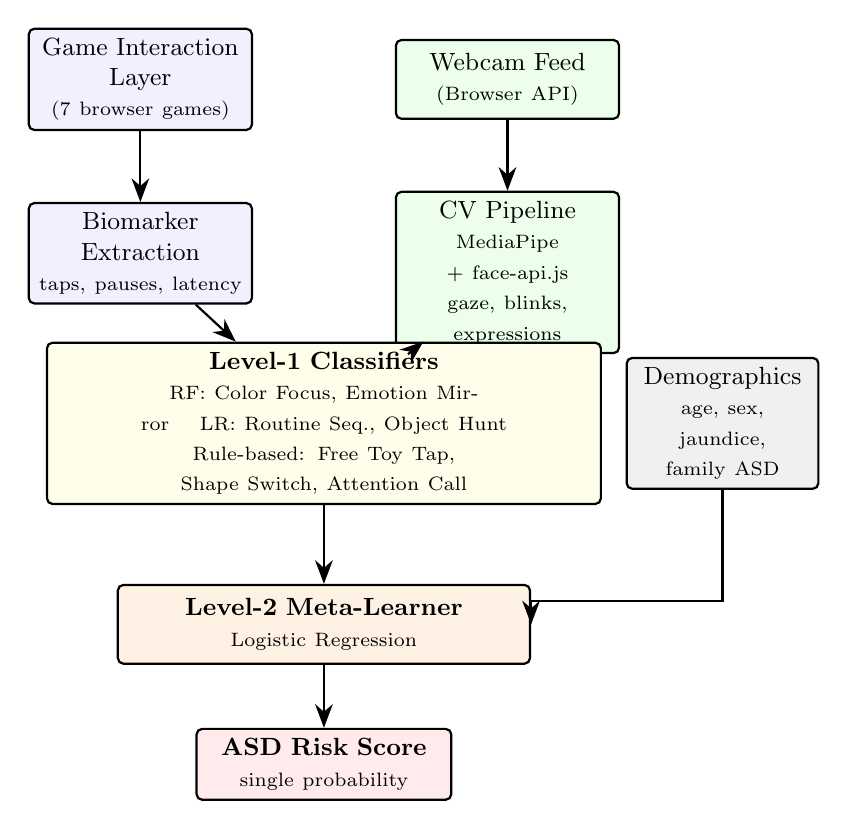
\begin{tikzpicture}[
    node distance=0.7cm and 1.2cm,
    every node/.style={font=\small},
    block/.style={rectangle, draw, thick, rounded corners=2pt, text width=2.6cm, minimum height=1cm, align=center, fill=blue!6},
    cvblock/.style={rectangle, draw, thick, rounded corners=2pt, text width=2.6cm, minimum height=1cm, align=center, fill=green!8},
    l1box/.style={rectangle, draw, thick, rounded corners=2pt, text width=6.8cm, minimum height=1.2cm, align=center, fill=yellow!8},
    demobox/.style={rectangle, draw, thick, rounded corners=2pt, text width=2.2cm, minimum height=0.8cm, align=center, fill=gray!12},
    metabox/.style={rectangle, draw, thick, rounded corners=2pt, text width=5.0cm, minimum height=1cm, align=center, fill=orange!10},
    outbox/.style={rectangle, draw, thick, rounded corners=2pt, text width=3.0cm, minimum height=0.9cm, align=center, fill=red!8},
    arr/.style={-{Stealth[length=3mm]}, thick}
]
% Top row
\node[block] (games) {Game Interaction\\Layer\\{\scriptsize (7 browser games)}};
\node[cvblock, right=1.8cm of games] (webcam) {Webcam Feed\\{\scriptsize (Browser API)}};

% Extraction row
\node[block, below=0.9cm of games] (bio) {Biomarker\\Extraction\\{\scriptsize taps, pauses, latency}};
\node[cvblock, below=0.9cm of webcam] (cv) {CV Pipeline\\{\scriptsize MediaPipe + face-api.js}\\{\scriptsize gaze, blinks, expressions}};

% Level 1
\node[l1box, below=1.0cm of $(bio)!0.5!(cv)$] (l1) {\textbf{Level-1 Classifiers}\\{\scriptsize RF: Color Focus, Emotion Mirror \quad LR: Routine Seq., Object Hunt}\\{\scriptsize Rule-based: Free Toy Tap, Shape Switch, Attention Call}};

% Demographics
\node[demobox, right=0.3cm of l1] (demo) {Demographics\\{\scriptsize age, sex, jaundice,}\\{\scriptsize family ASD}};

% Level 2
\node[metabox, below=1.0cm of l1] (l2) {\textbf{Level-2 Meta-Learner}\\{\scriptsize Logistic Regression}};

% Output
\node[outbox, below=0.8cm of l2] (out) {\textbf{ASD Risk Score}\\{\scriptsize single probability}};

% Arrows
\draw[arr] (games) -- (bio);
\draw[arr] (webcam) -- (cv);
\draw[arr] (bio) -- (l1);
\draw[arr] (cv) -- (l1);
\draw[arr] (l1) -- (l2);
\draw[arr] (demo.south) |- ([yshift=3mm]l2.east) -- (l2.east);
\draw[arr] (l2) -- (out);

\end{tikzpicture}%
}
\caption{NeuroStep pipeline overview. Game interactions and webcam-based facial analysis feed per-game Level-1 classifiers. Their outputs merge with demographic variables in a Level-2 meta-learner that produces one risk probability.}
\label{fig:architecture}
\end{figure}

\subsection{The Seven Games and What They Measure}
Each game targets a specific behavioral domain from the AQ-10 checklist. We capped every game at two minutes because pilot observations showed that children aged 4 to 8 lose focus past that mark. Table~\ref{tab:games} lists the AQ-10 items mapped to each game and the classifier type selected for it.

\begin{table}[htbp]
\caption{How Each Game Maps onto AQ-10 Domains}
\label{tab:games}
\centering
\renewcommand{\arraystretch}{1.15}
\begin{tabular}{@{}p{1.8cm}p{2.2cm}p{1.2cm}p{1.5cm}@{}}
\toprule
\textbf{Game} & \textbf{What It Targets} & \textbf{AQ-10 Items} & \textbf{L1 Model} \\
\midrule
Color Focus & Sustained attention, impulse control & A1, A2, A8 & Random Forest \\
Routine Seq. & Sequential planning & A3, A4 & Logistic Reg. \\
Emotion Mirror & Expression recognition, mimicry & A5, A6, A9 & Random Forest \\
Object Hunt & Visual discrimination & A7, A10 & Logistic Reg. \\
Free Toy Tap & Play diversity, repetitive patterns & A3, A4 & Rule-based \\
Shape Switch & Cognitive flexibility & A8 & Rule-based \\
Attention Call & Responding to name, gaze shift & A1, A5 & Rule-based \\
\bottomrule
\end{tabular}
\end{table}

\subsubsection{Color Focus Bubble Pop}
Multi-colored bubbles drift across the screen for 30 seconds. The child must pop only the blue ones. Two quantities are recorded:
\begin{itemize}
    \item \textbf{Score} $s$: correct (blue) pops
    \item \textbf{Errors} $e$: taps on wrong-color bubbles
\end{itemize}
When $e$ is high relative to $s$, the child is tapping impulsively without filtering by color. This pattern maps onto AQ-10 attention items A1, A2, and A8.

\subsubsection{Free Toy Tap}
Six animated toys sit on the screen for 75 seconds. There are no instructions at all; the child taps whatever they find interesting. We do not care about speed or accuracy here. What matters is whether taps spread evenly across the toys or cluster on just one or two.

\textit{Object Fixation Entropy.} Shannon entropy over the tap distribution:
\begin{equation}
H = -\sum_{i=1}^{N} p_i \log_2 p_i
\label{eq:entropy}
\end{equation}
$p_i$ is the fraction of taps on toy $i$. Entropy below 1.0 means the child stuck to one or two toys. Values above 2.5 mean the child sampled broadly. This distinction is important because repetitive, restricted behavior, including sustained fixation on one object, is a core DSM-5 criterion for ASD.

\textit{Repetition Rate.} The share of consecutive taps that land on the same toy. Values above 0.5 get flagged as repetitive play.

\textit{Switch Frequency.} How often the child moves from one toy to a different one. Rates below 0.15 point toward rigid play patterns.

\subsubsection{Attention Call}
Using the Web Speech API, the browser says the child's name out loud five times at irregular intervals during the session. After each call we check, via gaze tracking, whether the child looks toward the camera within 3.5 seconds. The response rate is computed as:
\begin{equation}
R_{response} = \frac{N_{looks}}{N_{calls}}
\label{eq:response_rate}
\end{equation}
Failure to respond to one's name is among the earliest observable indicators of ASD. Pediatricians already look for it in routine well-child visits; in many cases it is detectable before age two.

\subsubsection{Emotion Mirror}
A facial expression appears on screen (smile, surprise, or neutral) and the child tries to imitate it. Two vision models work in parallel. One judges whether the child's face actually matches the target expression. The other times two things: response latency, meaning how long the child takes to produce the expression, and expression stability, meaning how long they sustain it once produced. Mimicry was chosen on purpose. Clinical research going back more than ten years has documented that children on the autism spectrum take longer to initiate facial expressions and hold them for shorter periods compared to neurotypical peers.

\subsubsection{Shape Switch}
A target shape appears on screen and the child taps it. After every three correct taps the target switches without warning. Two quantities are tracked: perseveration errors (the child keeps tapping the old target after the rule changes) and confusion duration (time elapsed before the child begins hitting the new target). Both metrics reflect cognitive flexibility. Children with ASD tend to score poorly on both.

\subsection{Computer Vision Pipeline}

\subsubsection{Gaze Direction (MediaPipe Face Mesh)}
We estimate gaze direction by computing the iris position relative to the eye outline. The normalized offset is:
\begin{equation}
G_{offset} = \frac{|x_{iris} - x_{eye\_center}|}{w_{eye}}
\label{eq:gaze}
\end{equation}
$x_{iris}$ comes from landmarks 468 and 473 (iris centers). $x_{eye\_center}$ is the midpoint of the inner and outer canthi (landmarks 33, 133, 263, 362). $w_{eye}$ is the horizontal eye width. A value below 0.15 counts as eye contact.

\subsubsection{Eye Aspect Ratio (face-api.js)}
Blink detection follows the approach of Soukupov\'{a} and \v{C}ech~\cite{soukupova2016ear}:
\begin{equation}
EAR = \frac{\|p_2 - p_6\| + \|p_3 - p_5\|}{2 \cdot \|p_1 - p_4\|}
\label{eq:ear}
\end{equation}
$p_1$ through $p_6$ are the six eye-contour landmarks. An EAR above 0.22 means the eye is open; below that threshold the frame is classified as a blink or closed eye.

\subsubsection{Head Movement}
Nose-tip displacement between consecutive frames captures head motion:
\begin{equation}
M = \sqrt{(\Delta x_{nose})^2 + (\Delta y_{nose})^2}
\label{eq:movement}
\end{equation}
Displacements exceeding 0.03 count as active movement. We include this signal because repetitive or stereotyped head movements are among the motor behaviors sometimes seen in children with ASD.

\subsection{The Stacked Ensemble}

Our ensemble uses the stacked generalization framework of Wolpert~\cite{wolpert1992stacked}, adapted here for multi-game screening.

\subsubsection{Level 1: One Classifier per Game}
Four of the seven games are backed by trained classifiers. The other three rely on rule-based scoring.

\begin{itemize}
    \item \textbf{Color Focus} and \textbf{Emotion Mirror}: Random Forests with 50 trees and max depth of 5, trained on AQ-10 subsets $\{A1, A2, A8\}$ and $\{A5, A6, A9\}$.
    \item \textbf{Routine Sequencer} and \textbf{Object Hunt}: L2-regularized Logistic Regression on $\{A3, A4\}$ and $\{A7, A10\}$.
\end{itemize}

Free Toy Tap, Shape Switch, and Attention Call use rule-based scoring instead of learned models. The thresholds involved (entropy cutoffs, switch-rate boundaries, name-response counts) come from published clinical literature, and learned models did not improve over them in our preliminary experiments.

Each Level-1 component, learned or rule-based, outputs a calibrated probability $\hat{p}_k = P(y{=}1 \mid \mathbf{x}_k)$.

\subsubsection{Level 2: Meta-Learner}
One Logistic Regression model receives an 11-element input vector:
\begin{equation}
\mathbf{z} = [\hat{p}_1, \hat{p}_2, \ldots, \hat{p}_7, \text{age}, \text{gender}, \text{jaundice}, \text{family\_ASD}]
\label{eq:meta_features}
\end{equation}
Seven game-risk scores and four demographic variables. After standardization:
\begin{equation}
z_i^{*} = \frac{z_i - \mu_i}{\sigma_i}
\label{eq:scaling}
\end{equation}
the output is:
\begin{equation}
P(ASD \mid \mathbf{z}^{*}) = \sigma(\mathbf{w}^T \mathbf{z}^{*} + b) = \frac{1}{1 + e^{-(\mathbf{w}^T \mathbf{z}^{*} + b)}}
\label{eq:sigmoid}
\end{equation}
where $\mathbf{w} \in \mathbb{R}^{11}$ and bias $b$ are learned during training.

\subsubsection{Handling Missing Games}
Some children will not complete all seven games. A child might refuse one, get tired during another, or simply wander off. When a game goes unplayed, we fill its risk slot with the average risk from the games that were completed:
\begin{equation}
\hat{p}_{unplayed} = \frac{1}{|S_{played}|} \sum_{k \in S_{played}} \hat{p}_k
\label{eq:imputation}
\end{equation}
Zero-filling would understate risk. One-filling would overstate it. Averaging the played games is a neutral default.

\subsection{Training Data}
Training data came from two public sources:

\begin{enumerate}
    \item The \textbf{ASD Children Dataset} on the UCI repository, containing 292 records with 10 binary AQ-10 scores and demographic fields.
    \item A \textbf{Combined Autism Screening Dataset} that pools additional records under the same feature layout.
\end{enumerate}

We dropped exact duplicate rows and fixed encoding problems: yes/no fields had inconsistent casing, and the age column had been stored as a string type. After cleanup \textbf{5,519 records} survived, each carrying 14 features (ten AQ-10 items, age, gender, jaundice history, and family ASD history) plus a binary ASD label. We split 80/20 with stratification, giving 4,415 training and 1,104 test records. Ages were cast to floats, blanks filled with column means, gender encoded as 1/0, and yes/no fields binarized. Each feature subset was standardized on its own before being passed to its Level-1 model.

% ============================================================================
% IV. EXPERIMENTAL RESULTS
% ============================================================================
\section{Results and Discussion}

\subsection{Overall Performance}
Table~\ref{tab:global_results} reports classification metrics on the held-out test set of 1,104 records.

\begin{table}[htbp]
\caption{Classification Report for the Level-2 Meta-Learner}
\label{tab:global_results}
\centering
\renewcommand{\arraystretch}{1.2}
\begin{tabular}{@{}lccc@{}}
\toprule
\textbf{Class} & \textbf{Precision} & \textbf{Recall} & \textbf{F1-Score} \\
\midrule
No Risk        & 0.9500 & 0.9300 & 0.9400 \\
Risk Identified & 0.8500 & 0.8900 & 0.8700 \\
\midrule
\textbf{Accuracy}     & \multicolumn{3}{c}{\textbf{0.9185}} \\
\textbf{Macro Avg}    & 0.9000 & 0.9100 & 0.9000 \\
\textbf{Weighted Avg} & 0.9200 & 0.9200 & 0.9200 \\
\bottomrule
\end{tabular}
\end{table}

Look at the ``Risk Identified'' row. 85\% precision. Roughly one in six flagged children is a false positive, meaning the family gets referred when no referral was needed. That is annoying for those families. But we chose this trade-off deliberately. During training we tuned for recall, not precision, because the consequences of the two error types are wildly asymmetric. Missing a child who genuinely needs evaluation (false negative) is far worse than sending one extra neurotypical child to a specialist (false positive). The 89\% recall reflects this priority.

\subsection{Per-Game Performance}
No single game was designed to be a strong standalone classifier. Each covers a narrow slice of behavior. Table~\ref{tab:l1_results} shows their individual numbers.

\begin{table}[htbp]
\caption{Per-Game Classifier Accuracy}
\label{tab:l1_results}
\centering
\renewcommand{\arraystretch}{1.2}
\begin{tabular}{@{}lcccc@{}}
\toprule
\textbf{Game Model} & \textbf{Type} & \textbf{Acc.} & \textbf{Prec.} & \textbf{Rec.} \\
\midrule
Attention Call   & Rule  & 0.8265 & 0.7854 & 0.7124 \\
Emotion Mirror   & RF    & 0.8134 & 0.7529 & 0.5786 \\
Free Toy Tap     & Rule  & 0.7856 & 0.7123 & 0.6542 \\
Color Focus      & RF    & 0.7745 & 0.6930 & 0.4688 \\
Routine Seq.     & LR    & 0.7672 & 0.5922 & 0.7626 \\
Shape Switch     & Rule  & 0.7534 & 0.6845 & 0.5987 \\
Object Hunt      & LR    & 0.6884 & 0.4910 & 0.5668 \\
\bottomrule
\end{tabular}
\end{table}

Attention Call scored highest: 82.65\%. No surprise there. Name-response deficits are well documented as early ASD indicators~\cite{jones2013attention}. Object Hunt was weakest at 68.84\%, which suggests that visual discrimination by itself tells us little about ASD status. The important comparison is between the top single game and the combined ensemble: nine percentage points separate them (82.65\% versus 91.85\%). A game with mediocre standalone accuracy still contributes when stacked with the rest.

\subsection{Error Analysis}
Fig.~\ref{fig:confusion} breaks down the confusion matrix: 713 true negatives, 54 false positives, 299 true positives, 38 false negatives. 38 missed children out of 337 at-risk cases. That is an 11.3\% miss rate. Lower would be better, obviously. But we are talking about a browser-based screener with no clinician in the room. Catching every single case under those conditions is an unrealistic bar. For context, parent-report instruments carry comparable miss rates and add variance from subjective caregiver judgment on top of that. An 88.7\% detection rate looks reasonable to us.

\begin{figure}[htbp]
\centering
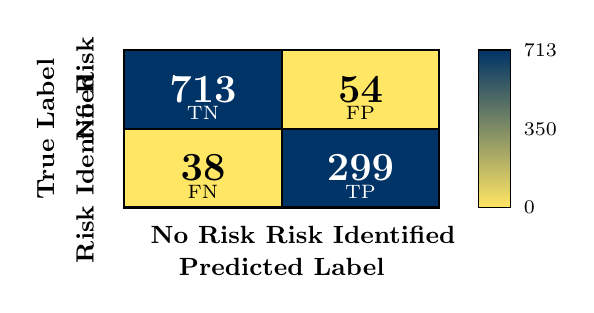
\begin{tikzpicture}[scale=1.0]
  % Define colors
  \definecolor{highval}{RGB}{0,51,102}
  \definecolor{lowval}{RGB}{255,230,100}
  % Draw cells with colors based on values
  % TN = 713 (high) - dark
  \fill[highval] (0,1) rectangle (2,2);
  \node[white,font=\Large\bfseries] at (1,1.5) {713};
  \node[white,font=\scriptsize] at (1,1.2) {TN};
  % FP = 54 (low) - light
  \fill[lowval] (2,1) rectangle (4,2);
  \node[black,font=\Large\bfseries] at (3,1.5) {54};
  \node[black,font=\scriptsize] at (3,1.2) {FP};
  % FN = 38 (low) - light
  \fill[lowval] (0,0) rectangle (2,1);
  \node[black,font=\Large\bfseries] at (1,0.5) {38};
  \node[black,font=\scriptsize] at (1,0.2) {FN};
  % TP = 299 (high) - dark
  \fill[highval] (2,0) rectangle (4,1);
  \node[white,font=\Large\bfseries] at (3,0.5) {299};
  \node[white,font=\scriptsize] at (3,0.2) {TP};
  % Grid lines
  \draw[thick] (0,0) rectangle (4,2);
  \draw[thick] (2,0) -- (2,2);
  \draw[thick] (0,1) -- (4,1);
  % X-axis labels (Predicted)
  \node[font=\small\bfseries] at (1,-0.35) {No Risk};
  \node[font=\small\bfseries] at (3,-0.35) {Risk Identified};
  \node[font=\small\bfseries] at (2,-0.75) {Predicted Label};
  % Y-axis labels (True)
  \node[font=\small\bfseries,rotate=90] at (-0.5,1.5) {No Risk};
  \node[font=\small\bfseries,rotate=90] at (-0.5,0.5) {Risk Identified};
  \node[font=\small\bfseries,rotate=90] at (-1.0,1.0) {True Label};
  % Color bar
  \shade[bottom color=lowval,top color=highval] (4.5,0) rectangle (4.9,2);
  \draw (4.5,0) rectangle (4.9,2);
  \node[font=\scriptsize,right] at (4.95,0) {0};
  \node[font=\scriptsize,right] at (4.95,1) {350};
  \node[font=\scriptsize,right] at (4.95,2) {713};
\end{tikzpicture}
\caption{Confusion matrix on the held-out test set ($n=1{,}104$). The 38 false negatives out of 337 risk cases represent the most critical failure mode of the system.}
\label{fig:confusion}
\end{figure}

\subsection{Meta-Learner Feature Importance}
Table~\ref{tab:coefficients} reports standardized coefficients from the Level-2 logistic regression.

\begin{table}[htbp]
\caption{Standardized Coefficients of the Level-2 Model}
\label{tab:coefficients}
\centering
\renewcommand{\arraystretch}{1.15}
\begin{tabular}{@{}lr@{}}
\toprule
\textbf{Feature} & \textbf{Coefficient} \\
\midrule
Emotion Mirror Risk      & 1.8923 \\
Attention Call Risk      & 1.6789 \\
Age                      & 1.5235 \\
Color Focus Risk         & 1.4961 \\
Routine Sequencer Risk   & 1.4659 \\
Object Hunt Risk         & 1.4105 \\
Shape Switch Risk        & 1.3457 \\
Gender                   & 0.1626 \\
Intercept                & $-2.5591$ \\
Jaundice History         & 0.0478 \\
Family ASD History       & 0.0412 \\
\bottomrule
\end{tabular}
\end{table}

Emotion Mirror and Attention Call dominate the ranking. Coefficients: 1.89 and 1.68 respectively. This is not a shock. Affect reciprocity and joint attention have been recognized as top-tier early ASD signals for decades. What is nice is that the model recovered this ranking entirely from data, with no manual weighting on our part. Gender barely matters (0.16). Jaundice history and family ASD history are both below 0.05. In practice the verdict comes almost exclusively from the child's in-game behavior, not from demographic background.

\subsection{Runtime Performance}
On the engineering side: React 19, Vite 7 for bundling, Firebase for auth plus Firestore, TensorFlow.js for the ML runtime, MediaPipe and face-api.js for vision. Framer Motion does the UI animations, Recharts the graphs, Zustand the state management. None of this is slow. The Level-2 sigmoid evaluation takes under a millisecond. The whole pipeline end to end, from collecting seven game scores through Level-1 inference to the meta-learner call, wraps up in under 50\,ms on a 2021 Intel i5 laptop. Parents get results the moment the last game finishes.

% ============================================================================
% V. CONCLUSION & FUTURE WORK
% ============================================================================
\section{Conclusion and Future Directions}

We set out to answer a simple question: can a webcam and fifteen minutes of browser games produce an ASD risk estimate that a family can act on? The numbers say probably yes. 91.85\% accuracy, 0.87 F1 on the risk class. We add ``probably'' because the caveats listed below are genuine.

What made the difference was stacking. The best individual game classifier hit 82.65\%. The full ensemble crossed 91\%. Checking attention in isolation or mimicry in isolation was never going to be enough. Probing seven behavioral domains and then letting a meta-learner figure out how to weight them, that is what pushed accuracy into a clinically useful range. The coefficient ranking lined up with clinical wisdom: social-emotional and joint-attention games carry the heaviest weight. The model found this on its own. Every computation happens on the user's machine. No installs, no uploads. A family on a bad internet connection sees exactly the same screener as one with gigabit fiber.

\subsection{Limitations}
The elephant in the data: we trained on questionnaire responses, not on recordings from children actually playing the games. Biomarkers were mapped to AQ-10 items through clinical reasoning, but no one has yet handed NeuroStep to a group of children and checked the output against proper ADOS-2 evaluations from licensed clinicians. Until that happens, accuracy figures in this paper are best treated as upper bounds. There is also the matter of the three rule-based games. Hand-tuned thresholds work for now, but they cannot catch finer behavioral patterns the way a learned model could.

\subsection{Future Work}
First priority: a \textbf{clinical validation trial}. Give NeuroStep to a real cohort of children, collect ADOS-2 scores from board-certified developmental pediatricians, and compare. Without that comparison the numbers we report are theoretical.

Second, we want to \textbf{swap the three rule-based classifiers for learned models} trained on raw interaction logs and webcam data. Fixed thresholds miss subtler patterns. A trained classifier with enough labeled examples could do better.

Third, Firebase already records session-level data per child. That makes \textbf{longitudinal monitoring} feasible: track risk scores over repeat visits, flag regression early. Building the feature is not hard. Getting families to come back for a second round, that is the real challenge.

% ============================================================================
% REFERENCES
% ============================================================================
\begin{thebibliography}{00}
\bibitem{lord2018autism}
C.~Lord, M.~Elsabbagh, G.~Baird, and J.~Veenstra-VanderWeele, ``Autism spectrum disorder,'' \textit{The Lancet}, vol.~392, no.~10146, pp.~508--520, 2018.

\bibitem{maenner2023prevalence}
M.~J.~Maenner \textit{et~al.}, ``Prevalence and characteristics of autism spectrum disorder among children aged 8 years,'' \textit{MMWR Surveill. Summ.}, vol.~72, no.~2, pp.~1--14, 2023.

\bibitem{zwaigenbaum2015early}
L.~Zwaigenbaum \textit{et~al.}, ``Early identification of autism spectrum disorder: Recommendations for practice and research,'' \textit{Pediatrics}, vol.~136, no.~Suppl.~1, pp.~S10--S40, 2015.

\bibitem{robins2014mchat}
D.~L.~Robins, D.~Fein, and M.~L.~Barton, ``The Modified Checklist for Autism in Toddlers, Revised with Follow-Up (M-CHAT-R/F),'' \textit{Pediatrics}, vol.~133, no.~1, pp.~37--45, 2014.

\bibitem{allison2012aq10}
C.~Allison, B.~Auyeung, and S.~Baron-Cohen, ``Toward brief `Red Flags' for autism screening: The Short Autism Spectrum Quotient and the Short Quantitative Checklist for Autism in Toddlers,'' \textit{J.~Am.~Acad.~Child Adolesc.~Psychiatry}, vol.~51, no.~2, pp.~202--212, 2012.

\bibitem{lord2012ados}
C.~Lord \textit{et~al.}, ``Autism Diagnostic Observation Schedule, Second Edition (ADOS-2),'' Torrance, CA: Western Psychological Services, 2012.

\bibitem{thabtah2019ml}
F.~Thabtah, ``Machine learning in autistic spectrum disorder behavioral research: A review and ways forward,'' \textit{Informatics for Health and Social Care}, vol.~44, no.~3, pp.~278--297, 2019.

\bibitem{duda2016clinical}
M.~Duda, R.~Ma, N.~Haber, and D.~P.~Wall, ``Use of machine learning for behavioral distinction of autism and ADHD,'' \textit{Transl.~Psychiatry}, vol.~6, no.~2, p.~e732, 2016.

\bibitem{li2019facial}
J.~Li, G.~Zhong, and C.~Xu, ``Facial expression recognition with deep learning,'' in \textit{Proc.~ACM Int.~Conf.~Multimedia}, 2019, pp.~2851--2854.

\bibitem{wang2019autism}
Q.~Wang \textit{et~al.}, ``Autism screening using deep neural network and eye tracking data,'' in \textit{Proc.~IEEE Int.~Conf.~Bioinformatics Biomed.~(BIBM)}, 2019, pp.~1028--1032.

\bibitem{murias2018jake}
M.~Murias, S.~Major, S.~Davlantis, L.~Franz, A.~Harris, B.~Rardin, M.~Sabatos-DeVito, and G.~Dawson, ``Validation of eye-tracking measures of social attention as a biomarker for autism,'' \textit{Autism Res.}, vol.~11, no.~1, pp.~166--174, 2018.

\bibitem{dawson2018autismbeyond}
G.~Dawson \textit{et~al.}, ``Atypical postural control can be detected via computer vision analysis in toddlers with autism spectrum disorder,'' \textit{Sci.~Rep.}, vol.~8, p.~17008, 2018.

\bibitem{lugaresi2019mediapipe}
C.~Lugaresi \textit{et~al.}, ``MediaPipe: A framework for building perception pipelines,'' in \textit{Proc.~Workshop on ML for Mobile}, 2019.

\bibitem{jones2013attention}
W.~Jones and A.~Klin, ``Attention to eyes is present but in decline in 2--6-month-old infants later diagnosed with autism,'' \textit{Nature}, vol.~504, pp.~427--431, 2013.

\bibitem{wolpert1992stacked}
D.~H.~Wolpert, ``Stacked generalization,'' \textit{Neural Networks}, vol.~5, no.~2, pp.~241--259, 1992.

\bibitem{soukupova2016ear}
T.~Soukupov\'{a} and J.~\v{C}ech, ``Eye blink detection using facial landmarks,'' in \textit{Proc.~21st Comput.~Vis.~Winter Workshop (CVWW)}, 2016.

\end{thebibliography}

\end{document}